\section*{Questão 1}
% Enunciado
\noindent {\it Um sistema com realimentação unitária tem a seguinte função de
transferência de malha aberta:}

\begin{equation}\nonumber
G(s) = \frac{9}{s(s+p)}
\end{equation}

\noindent {\it em que $p$ é normalmente igual a 3. Determine a sensibilidade da
função de transferência de malha fechada $T(s)$ em relação ao parâmetro $p$ e
plote os diagramas de Bode (módulo e fase) para $p$ variando entre 1 e 5.
Analise os resultados.}

\vspace{0.5cm}

\noindent{\bf Resolução:}

\vspace{0.25cm}

Antes de realizar a análise da sensibilidade em malha fechada, deve-se verificar
a estabilidade relativa do sistema em malha aberta quanto à variação do
parâmetro $p$. 

Sabe-se que essa estabilidade relativa pode ser observada a partir de duas
medidas dos diagramas de Bode, denominadas {\it margem de ganho} e {\it margem
de fase}. Para \citeasnoun{dorf:2009}, a {\it margem de ganho} é definida como
um acréscimo no ganho do sistema quando a fase é igual a -180\textdegree,
resultando em um sistema marginalmente estável, enquanto que a {\it margem de
fase} é definida como a quantidade de deslocamento de fase com magnitude
unitária que resultará em um sistema marginalmente estável.

Assim sendo, ao se observar a Fig. \ref{fig:bode_ma}, verifica-se que essas duas
medidas variam conforme Tab. \ref{tab:margem_ganho_fase_ma} para o sistema em
malha aberta\footnote{Apesar dos diagramas de Bode exibidos ao longo de toda a
resolução estarem sendo referenciados às equações no domínio de {\it Laplace}
com a variável complexa $s$, obter equações no domínio da frequência resume-se a
substituir a variável $s$ por $j\omega$.}.

\begin{figure}[htb]
\centering
    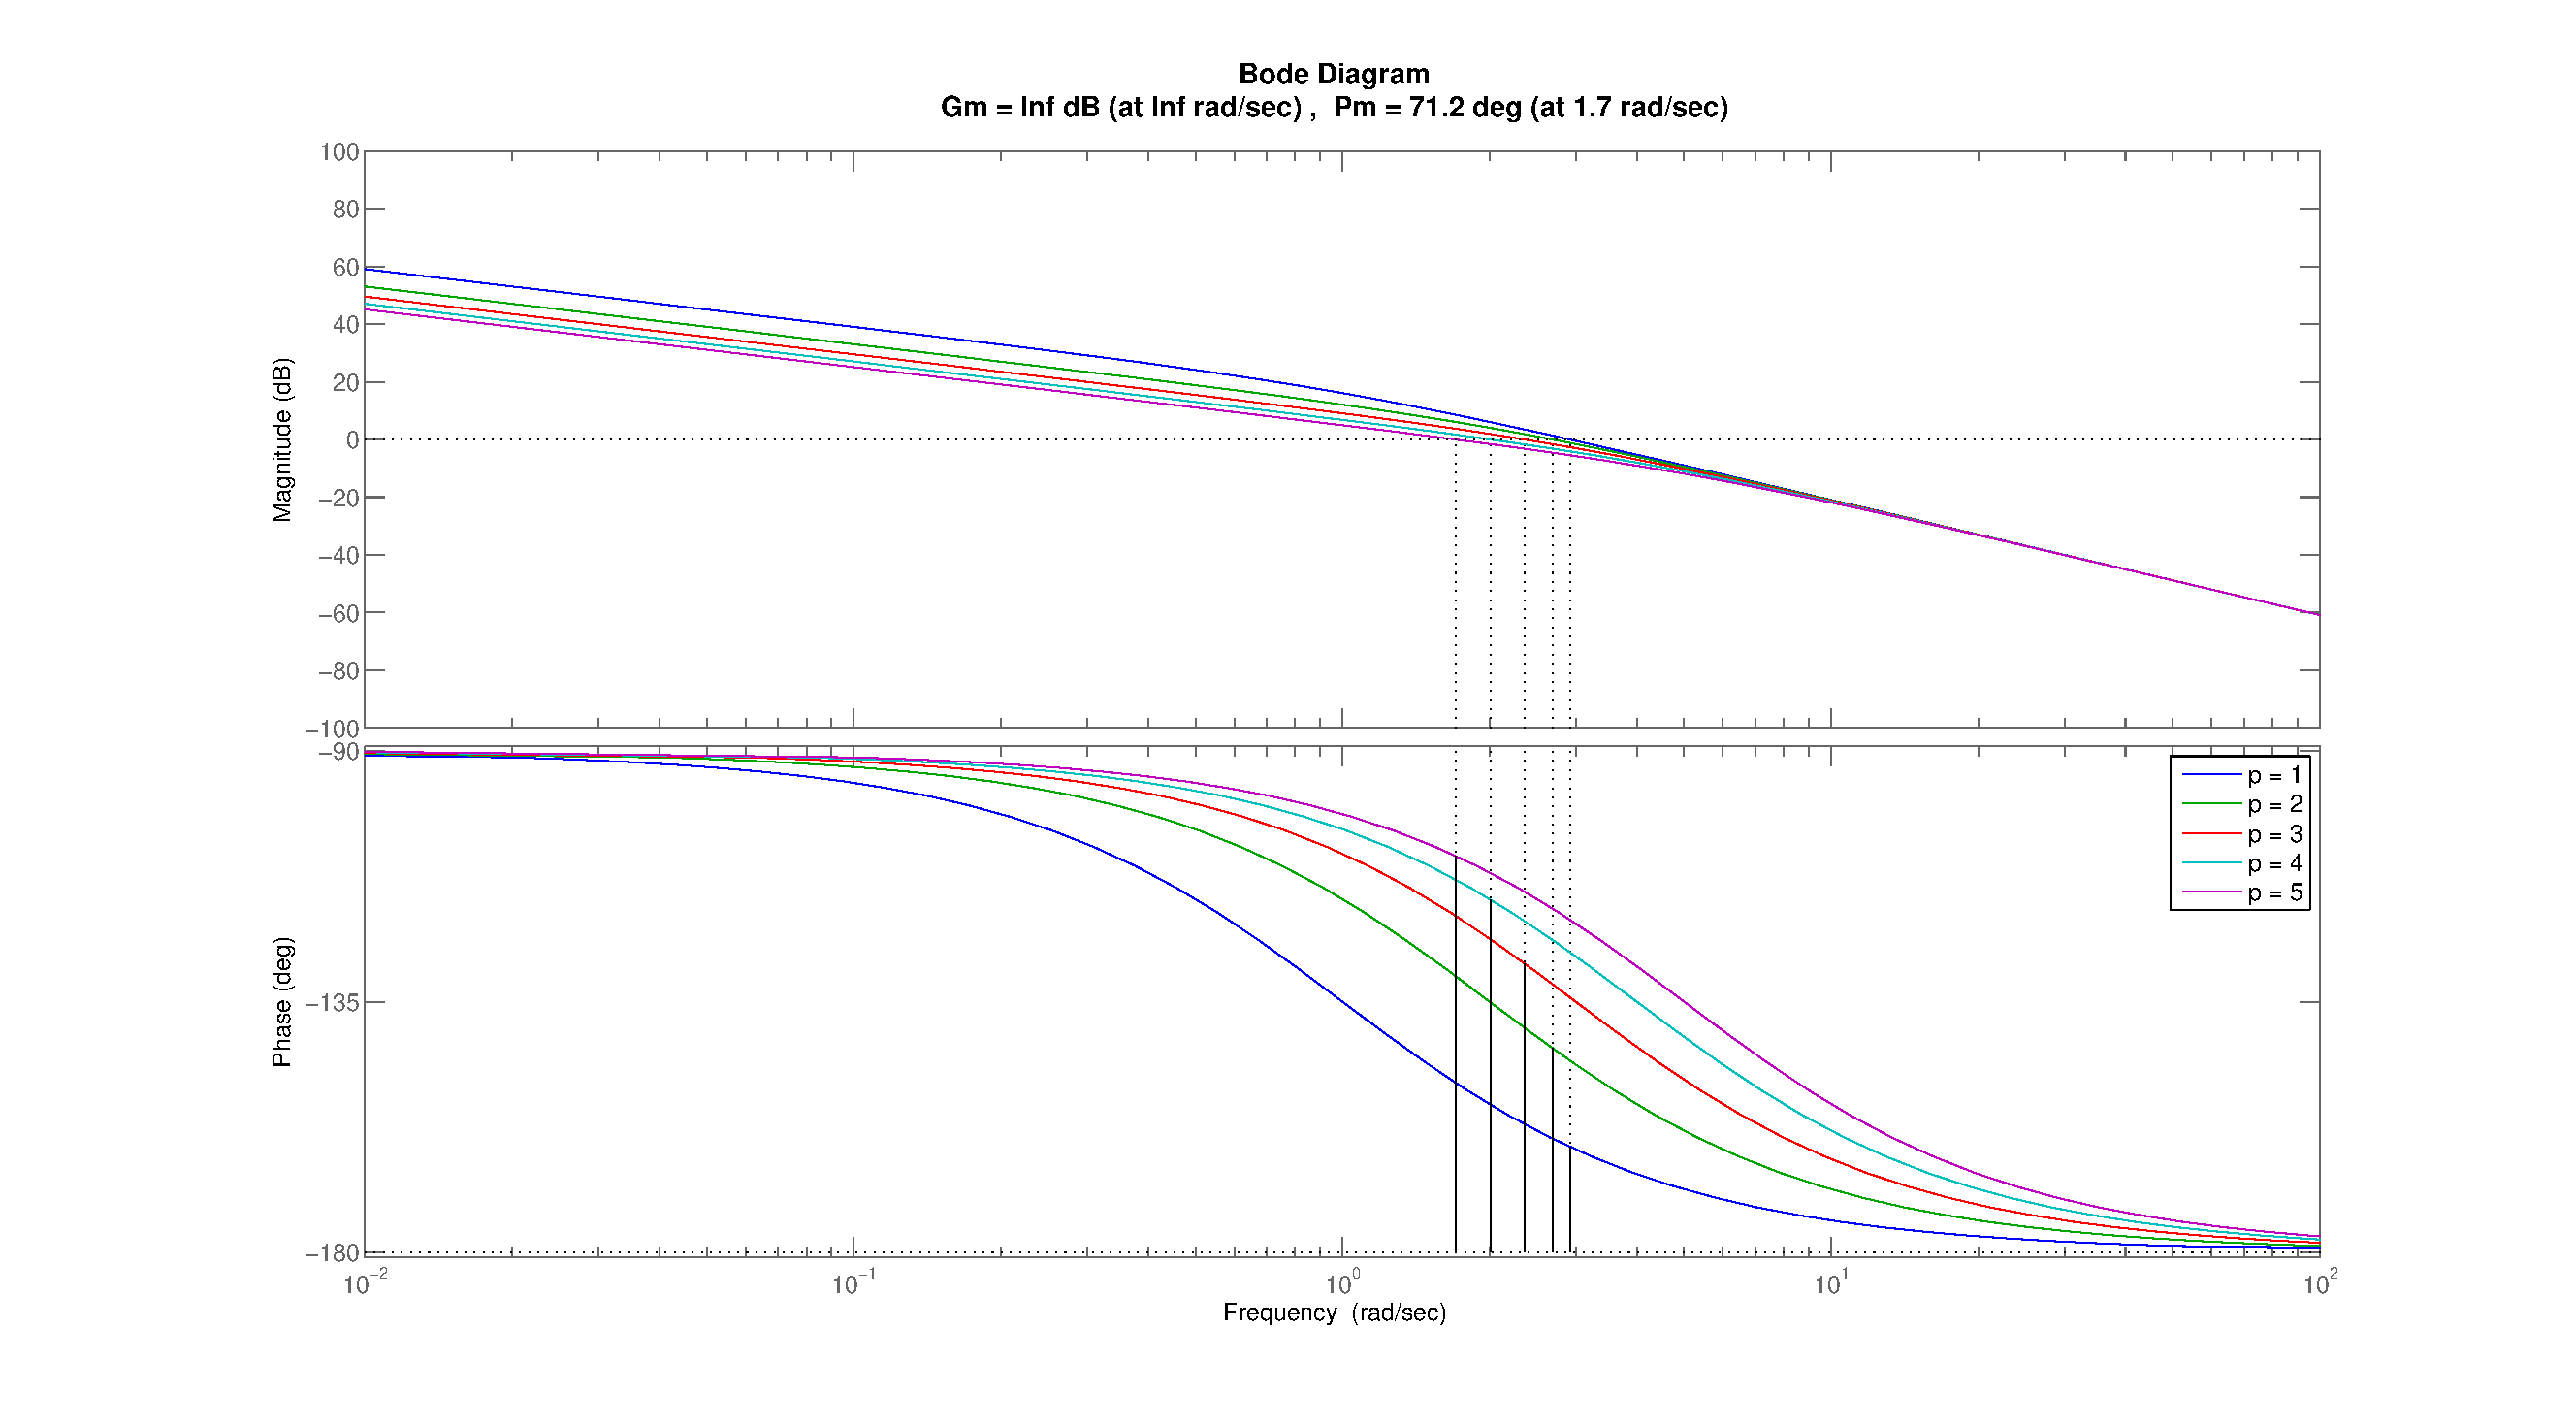
\includegraphics[width=0.95\textwidth]{imgs/questao1/bode_ma}
    \caption{Diagrama de bode para o sistema em malha aberta.}
    \label{fig:bode_ma}
\end{figure}

\begin{table}
\centering
    \caption{Margem de ganho e margem de fase para o sistema em malha aberta.}
    \label{tab:margem_ganho_fase_ma}
    \vspace{0.25cm}
\begin{tabular}{|c|c|c|c|c|}
\hline
$p$ & Margem de Ganho (MG) & $\omega_\text{MG}$ & 
Margem de Fase (MF) & $\omega_\text{MF}$\\
\hline
\hline
1 & $\infty$ & $\infty$ & 18.9175 & 2.9179\\
\hline
2 & $\infty$ & $\infty$ & 36.6620 & 2.6869\\
\hline
3 & $\infty$ & $\infty$ & 51.8273 & 2.3585\\
\hline
4 & $\infty$ & $\infty$ & 63.3162 & 2.0104\\
\hline
5 & $\infty$ & $\infty$ & 71.1830 & 1.7038\\
\hline
\end{tabular}
\end{table}

Sabendo que o sistema será estável quando a margem de ganho e a margem de fase
forem positivas, percebe-se que para os valores de $p = 1\text{,}\ 2\text{,}\ 
\ldots\text{,}\ 5$, o sistema é estável.

Dessa maneira, deseja-se agora realizar a análise em malha fechada. Para isso, a
função de transferência de malha fechada pode ser obtida a partir da Eq.
\ref{eq:G_MF}:

\begin{equation}\label{eq:G_MF}
G_{MF}(s) = \frac{G(s)}{1+G(s)H(s)}
\end{equation}

\noindent na qual $G(s)$ é função de transferência de malha aberta e $H(s)$ a
função de transferência do bloco da realimentação, conforme Fig.
\ref{fig:diag_bloco}. Assim sendo, a função de transferência de malha fechada
para o sistema do enunciado com realimentação unitária é dada pela Eq.
\ref{eq:G_MF_q1}:

\begin{figure}[htb]
\centering
    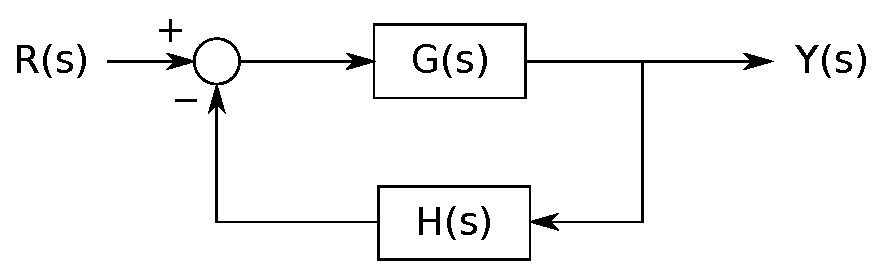
\includegraphics[width=0.55\textwidth]{imgs/questao1/diag_bloco}
    \caption{Diagrama de blocos de um sistema realimentado.}
    \label{fig:diag_bloco}
\end{figure}

\begin{eqnarray}
G_{MF}(s) & = & \frac{G(s)}{1+G(s)H(s)}\nonumber\\
          & = & \frac{G(s)}{1+G(s)}\nonumber\\
          & = & \frac{\D\frac{9}{s(s+p)}}{1+\D\frac{9}{s(s+p)}}\nonumber\\
          & = & \frac{\D\frac{9}{s(s+p)}}{\D\frac{s(s+p)+9}{s(s+p)}}\nonumber\\
          & = & \frac{9}{s(s+p)+9}\nonumber\\
          & = & \frac{9}{s^2 + ps + 9}\label{eq:G_MF_q1}
\end{eqnarray}

Observando a Fig. \ref{fig:bode_mf}, percebe-se que o sistema possuirá um
comportamento oscilatório característico das curvas com picos no diagrama de
Bode. Tal comportamento é comprovado a partir da resposta ao degrau unitário,
conforme Fig. \ref{fig:resp_deg_mf}.

\begin{figure}[htb]
\centering
    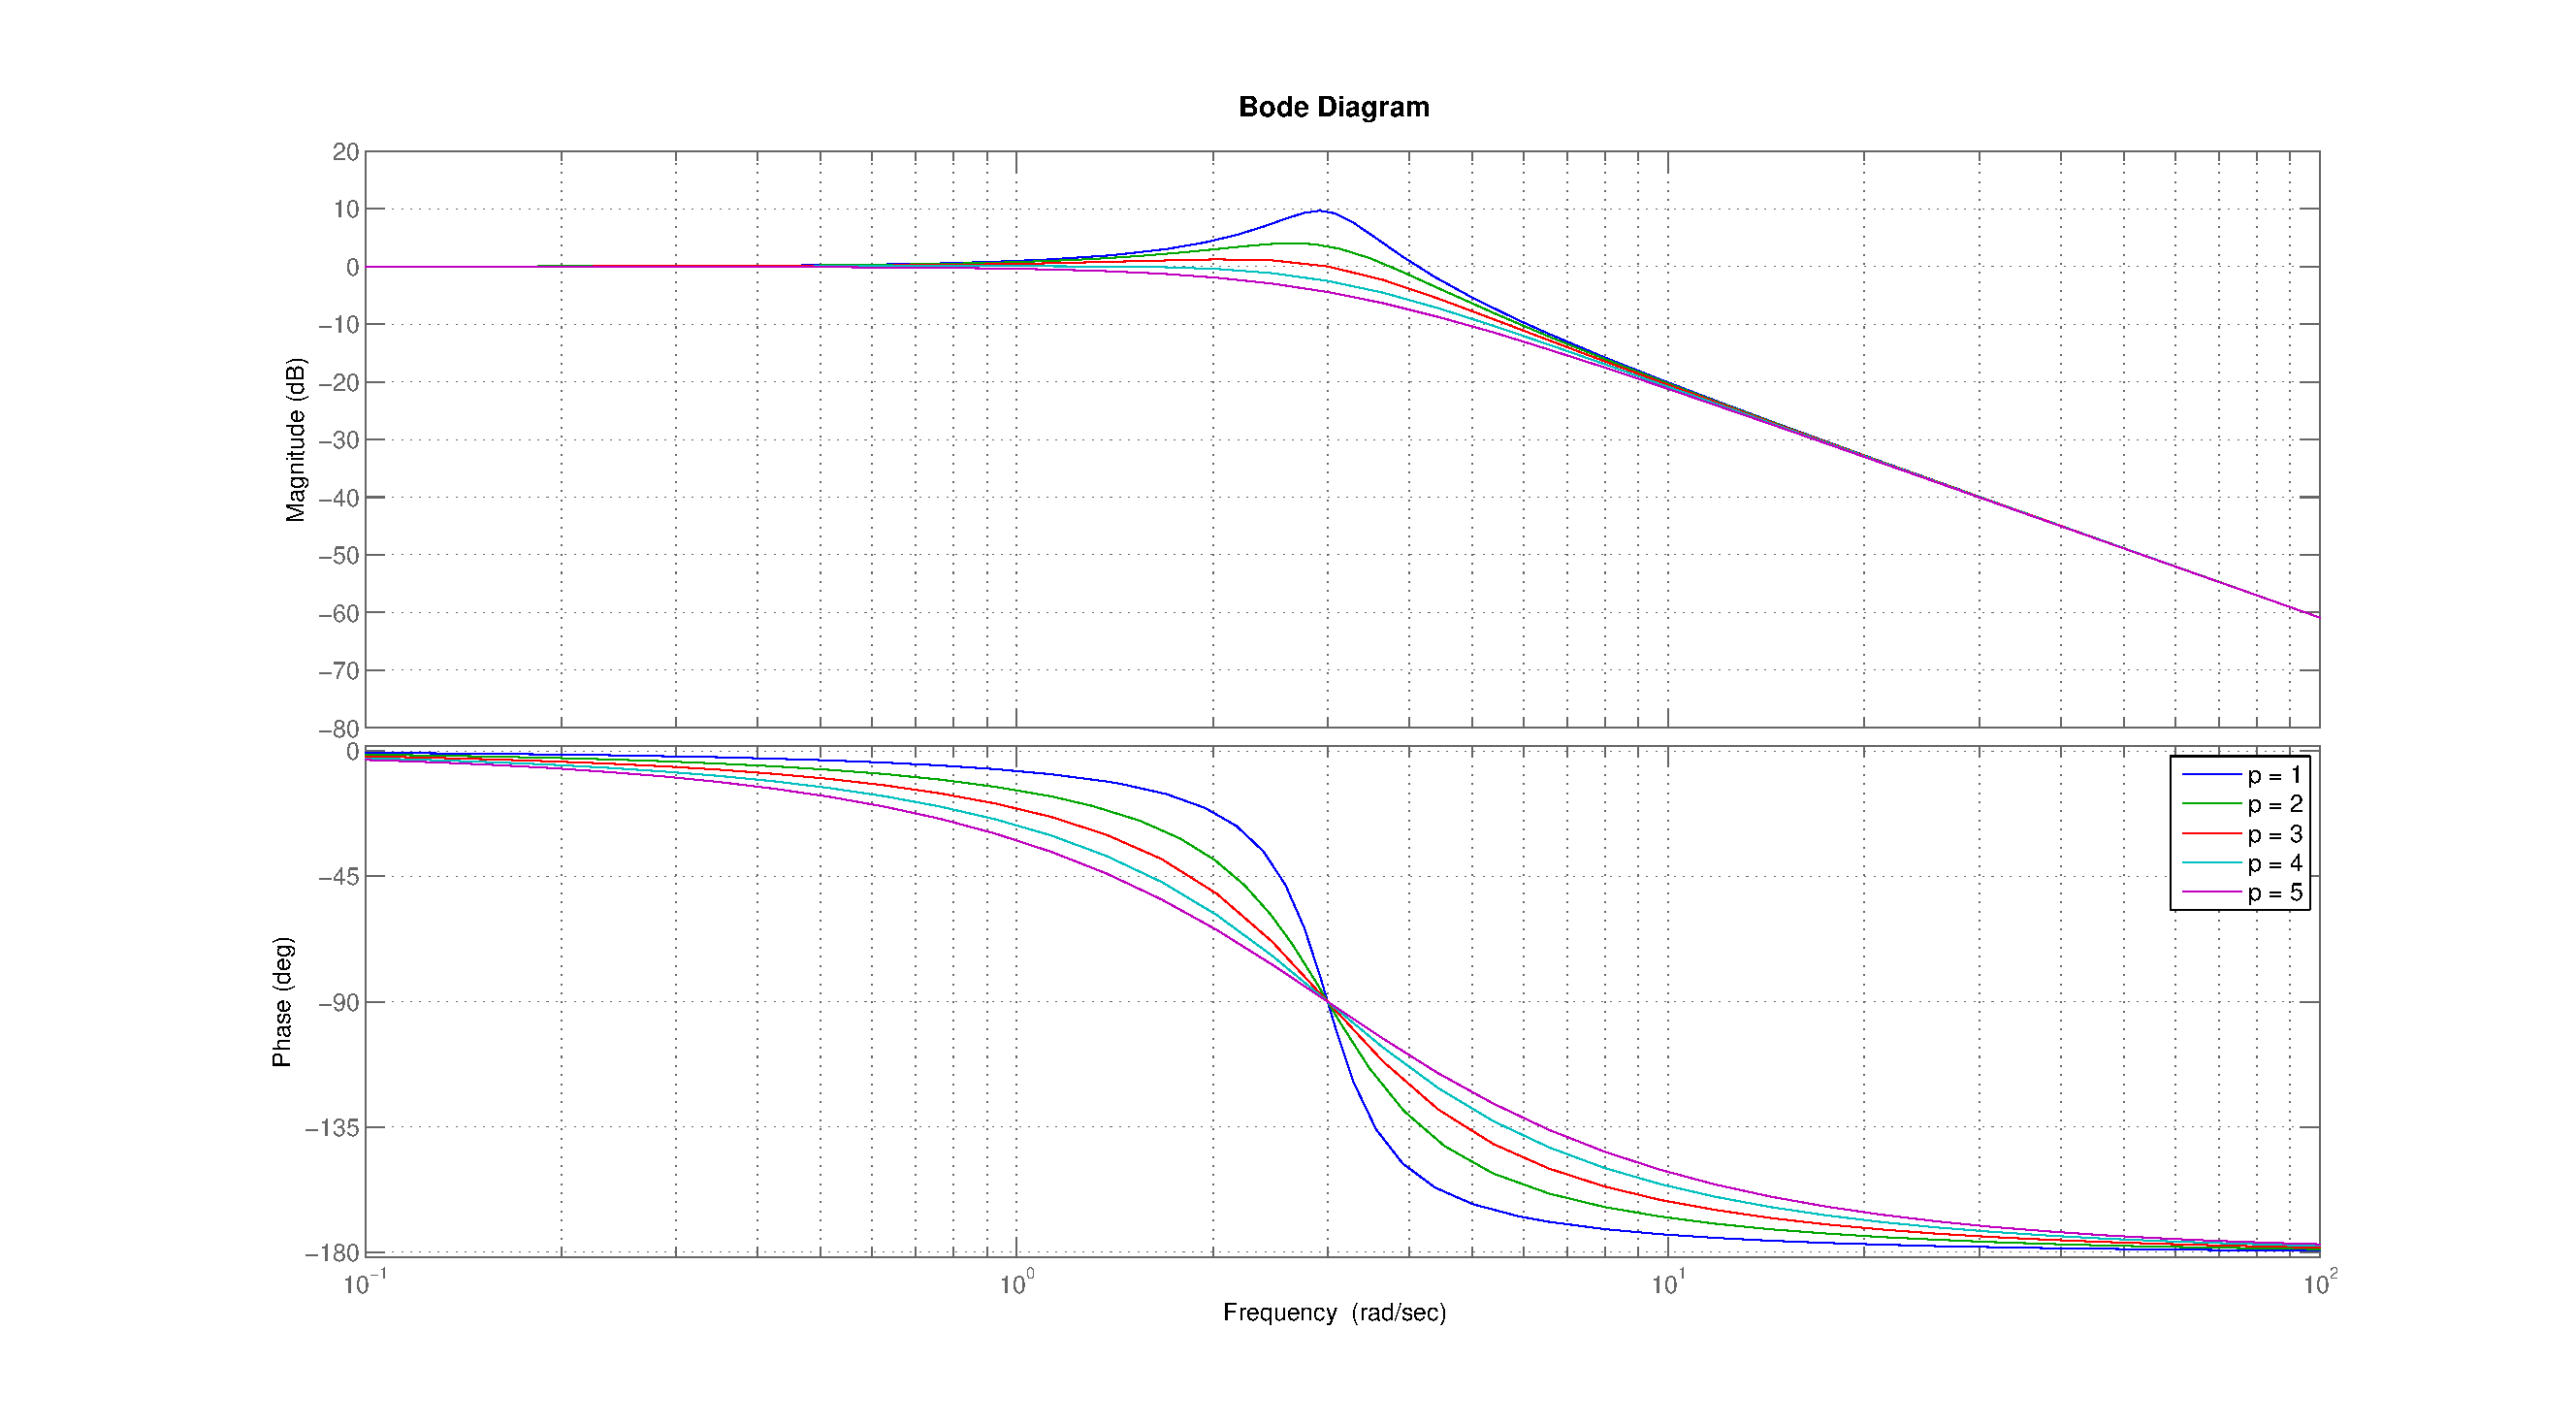
\includegraphics[width=0.95\textwidth]{imgs/questao1/bode_mf}
    \caption{Diagrama de bode para o sistema em malha fechada.}
    \label{fig:bode_mf}
\end{figure}

\begin{figure}[htb]
\centering
    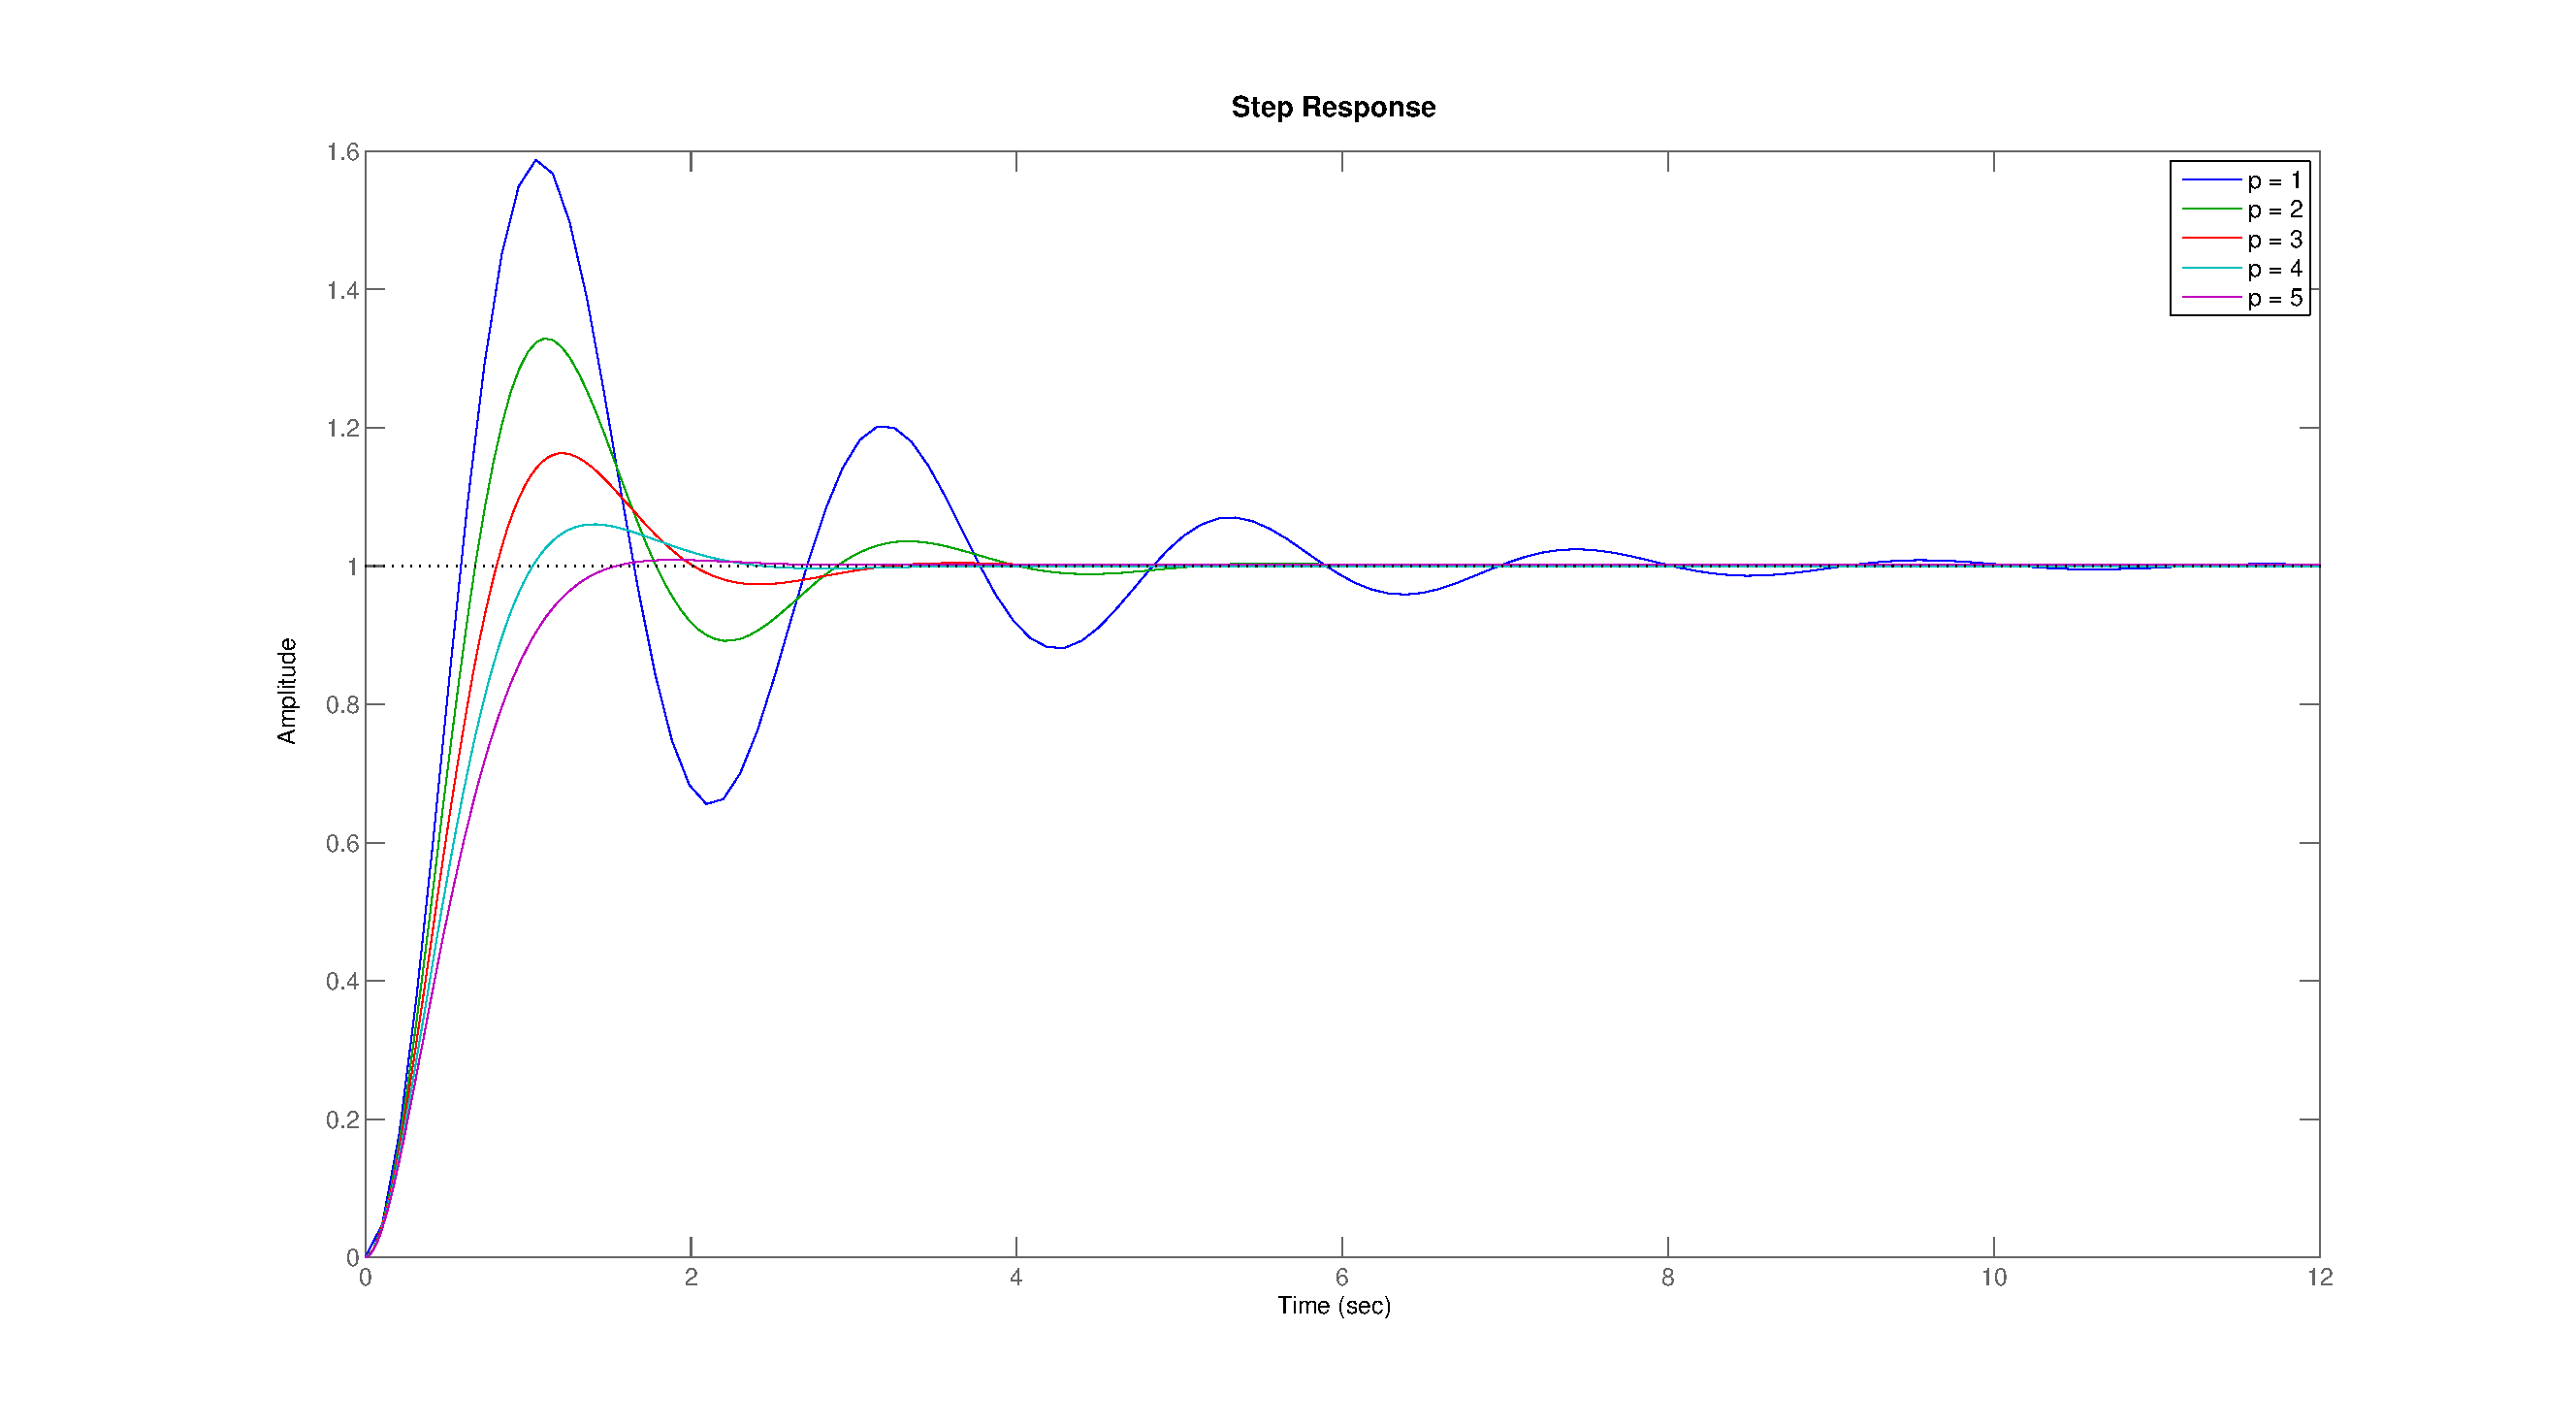
\includegraphics[width=0.95\textwidth]{imgs/questao1/resp_deg_mf}
    \caption{Resposta ao degrau unitário do sistema em malha fechada.}
    \label{fig:resp_deg_mf}
\end{figure}

Para \citeasnoun{dorf:2009}, a sensibilidade de um sistema é definida como sendo
a razão entre a variação percentual da função de transferência do sistema e a
variação percentual da função de transferência do processo (ou parâmetro). Ou
seja, para uma dada função de transferência do sistema $T(s)$, tem-se:

\begin{equation}
S = \frac{\Delta T(s)/T(s)}{\Delta G(s)/G(s)}
\end{equation}

No limite, para pequenas variações incrementais, tem-se:

\begin{equation}
S_G^T(s) = \frac{\partial T / T}{ \partial G / G} 
         = \frac{\partial T}{\partial G} \cdotp \frac{G}{T}
\end{equation}

Assim, para o parâmetro $p$ da função de transferência de malha fechada
obtida pela Eq. \ref{eq:G_MF_q1}, tem-se:

\begin{eqnarray}
S_p^G(s) & = & \frac{\partial G}{\partial p} \cdotp \frac{p}{G}\nonumber \\
         & = & \frac{0(s^2 + ps + 9) - 9(s)}{(s^2 + ps + 9)^2} \cdotp
               \frac{p}{\D\frac{9}{s^2 + ps + 9}}\nonumber\\
         & = & - \frac{9ps}{9(s^2 + ps + 9)}\nonumber\\
         & = & - \frac{ps}{s^2 + ps + 9}\label{eq:sensib}
\end{eqnarray}

Considerando $p = 1\text{,}\ 2\text{,}\ \ldots\text{,}\ 5$, obtém-se os
diagramas de Bode ilustrados pela Fig. \ref{fig:diag_bode_sensib}.

\begin{figure}[H]
\centering
    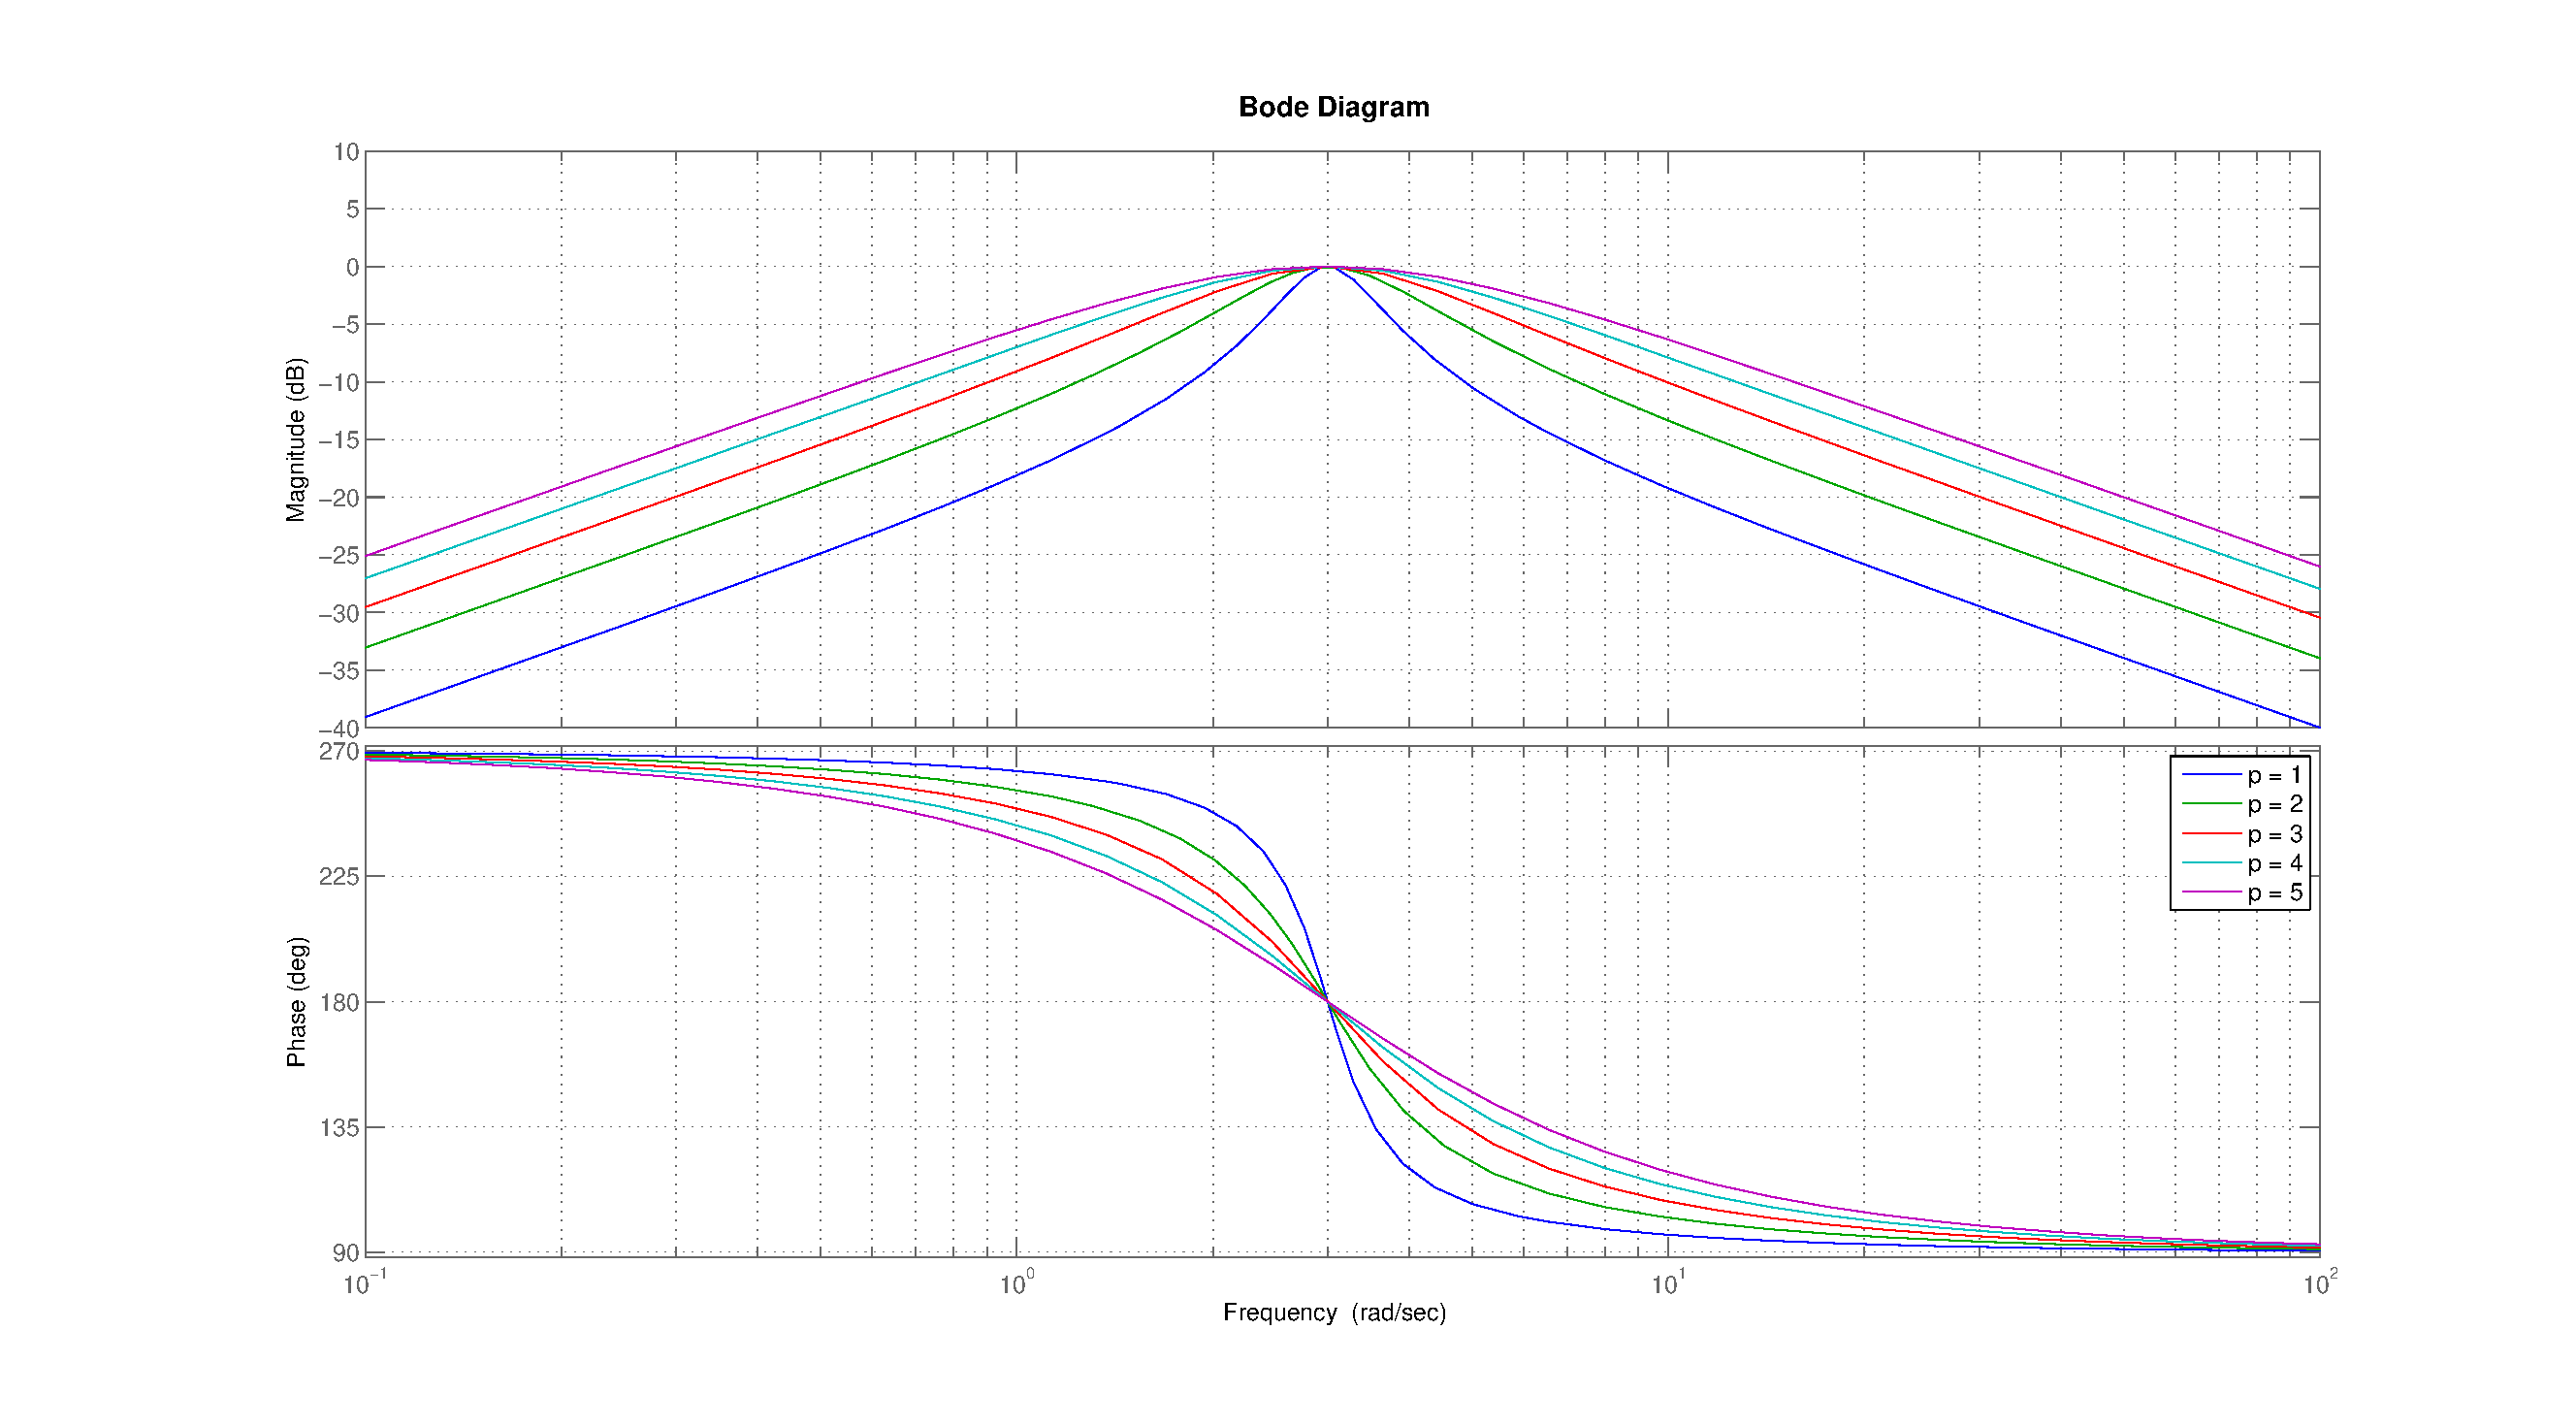
\includegraphics[width=0.95\textwidth]{imgs/questao1/bode_sensib}
    \caption{Diagrama de bode para a Eq. \ref{eq:sensib}.}
    \label{fig:diag_bode_sensib}
\end{figure}

Tendo em vista que os sistemas robustos são aqueles que apresentam baixa
sensibilidade à variação dos parâmetros, pode-se dizer que, para os sistemas
mais robustos, a sensibilidade ideal é tão baixa quanto possível.

Analisando então as curvas de módulo da Fig. \ref{fig:diag_bode_sensib},
verifica-se que todas elas apresentam baixa sensibilidade para frequências
baixas e altas. Entretanto, observa-se uma equivalência quanto a sensibilidade
para frequências em torno de 3 rad/s.

Fazendo uma análise comparativa, pode-se dizer que o sistema é estável para a
faixa de variação do parâmetro $p$ e que apresenta maior robustez quando $p =
1$, pois é a curva que apresenta os menores valores dentre as curvas de módulo
do diagrama de Bode. Contudo, observa-se que o sistema se torna bastante
oscilatório para esse valor de $p$, o que era esperado, uma vez que a relação
desempenho/robustez é inversa.

O {\it script} do Matlab\textsuperscript{\textregistered} desenvolvido para a
resolução dessa questão pode ser encontrado no Apêndice \ref{ap:cod_q1}.
